\begin{td}{Électrostatique}
\exercice{Potentiel de Yukawa}
	Le physicien japonais Yukawa a postulé la forme d'un potentiel pour modéliser
	les interactions entre particules dans un noyau atomique. Nous étudions
	ici ce potentiel comme s'il s'agissait d'un potentiel électrostatique.

	Dans un repère sphérique $(\er, \ephi, \etheta)$, une distribution de 
	charge à symétrie sphérique crée, à une distance $r$,
	un potentiel électrostatique de la forme
	\begin{equation}
		V(r) = \dfrac{Q}{4 \pi \epsilon_0 r} \exp\left(-\dfrac{r}{a}\right),
	\end{equation}
	$Q$ et $a$ étant des constantes positives.

	\begin{enumerate}
		\item Déterminer les unités de $Q$ et de $a$.
		\item Déterminer le champ électrostatique correspondant.
		\item En déduire la charge $q(r)$ contenue dans une sphère de 
		  rayon $r$ et de centre $O$.
		\item Déterminer $q(r)$ dans les deux cas extrêmes
			\begin{enumerate}
				\item $r$ tend vers zéro,
				\item $r$ tend vers $\infty$
			\end{enumerate}
		 En déduire qualitativement la nature de la distribution de charge
		 et donner une interprétation de $a$.
 	\end{enumerate}


\exercice{Champ gravitationnel dans une cavité}
Un modèle de Terre de rayon $R_1$ et de centre $O_1$ possède une masse volumique 
$\rho>0$ uniforme sauf dans une cavité sphérique, 
entièrement incluse dans la boule, centrée en $O_2$, de rayon $R_2$
(voir Fig~\ref{fig:cavite}). 

On cherche le champ gravitationnel $\vecg(M)$ en un point $M$ 
à l'intérieur de la cavité.
Dans un premier temps, on ignore la présence de la cavité.
\begin{enumerate}
	\item Rappeler l'expression du champ électrostatique $\vece$ générée par une
	  charge $q$ et du champ gravitationnel $\vecg$ générée par une particule
	  de masse $m$ en un point $P$ de l'espace. 
	  En déduire un tableau d'analogie entre interaction
	  gravitationnelle et interaction coulombienne.
  	\item En déduire un théorème de Gauss pour le champ gravitationnel
	  $\vecg$.
	\item Étudier les symétries et invariances du système en l'absence de
	  la cavité creuse.
	\item En appliquant le théorème de Gauss, déterminer l'expression
	  du champ $\vecg$ en un point $M$ de l'espace.
	  Vérifier l'homogénéité de l'expression obtenue.
	\item Étudier les symétries et invariances du système avec la cavité.
	  Pensez-vous qu'il soit judicieux d'utiliser le théorème de Gauss
	  ici ?
	\item En vous servant du théorème de superposition, 
	  déterminer le champ $\vecg$ en un point $M$ à l'intérieur de la cavité.
\end{enumerate}

\begin{figure}[h!]
\centering
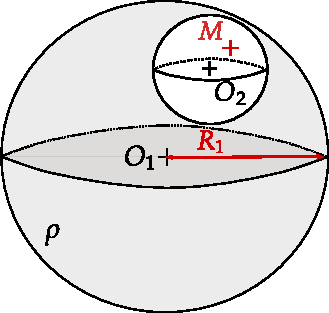
\includegraphics[scale = 0.6]{cavite.pdf}
\caption{Schéma de la sphère de masse volumique $\rho$ (en gris sur le schéma) 
	 et de la cavité vide (en blanc).
         À l'intérieur de la cavité, la masse volumique vaut 0.}
\label{fig:cavite}
\end{figure}

\exercice{Fil chargé}
	Calculer le champ électrostatique créé par un fil rectiligne infini
	uniformément chargé avec une densité linéïque de charge $\lambda$, en 
	tout point de l'espace.

\end{td}
